\section{Preliminary Study}
\label{sec:preStudy}

% Motivation and study questions
Existing studies have shown that ambiguous, noisy, or incomplete requirements can degrade the performance of code generation models~\cite{vijayvargiya2026ambigsweinteractiveagentsovercome,10554837,mu2024clarifygpt,jia2025specfix}. While several studies have investigated the impact of various uncertainty factors, such as clarity, typographical errors, and the presence or absence of examples~\cite{10.1145/3697010,liu2024trustworthyllmssurveyguideline,DBLP:journals/corr/abs-2406-10101,xia-etal-2025-survey}, their primary evaluation metric has been the test-case passing rate. In this preliminary study, we aim to explore how these factors affect the reliability of code generation.

%Perturbation design and dataset construction
\noindent\textbf{Study Setup.} Our preliminary study follows a three-step pipeline. We first collect perturbation types from prior studies on natural-language perturbation, prompt robustness, and requirements ambiguity, as summarized in Table~\ref{tab:uncertainty_factors}. We then inject these perturbations into the requirement descriptions of public benchmarks to construct perturbed inputs. Finally, we evaluate the quality and stability of generated code under these perturbed requirements. Specifically, we use HumanEval-ET, the extended-test version of HumanEval from EvalPlus~\cite{humaneval,liu2023evalplus}, as a controlled function-level testbed. We further include LiveCodeBench~\cite{jain2025livecodebench} as a more challenging benchmark to examine whether the observed effects generalize beyond HumanEval-style prompts.

%explain the purbation types
Referring to the existing literature, the perturbation process combines LLM-assisted rewriting, rule-based transformation, and TextAttack-based character transformation~\cite{morris2020textattack}. Specifically, content rewriting and format transformation are generated through LLM-assisted rewriting, where they require preserving the original task intent while changing the semantic expression or presentation style of the requirement. For content rewriting, the LLM is prompted to paraphrase or abstract detailed expressions of functional constraints, edge cases, or task intent. For format transformation, the LLM rewrites the requirement into a more natural and conversational paragraph while preserving the original functional requirements and constraints. Example removal, verbose rewriting, and noise injection are implemented using rule-based transformations. Example removal deletes input-output examples from the original prompt, such as doctest-style examples in HumanEval-style tasks and sample input-output cases in programming-contest-style tasks. Verbose rewriting adds redundant explanatory descriptions, while noise injection appends task-irrelevant natural-language sentences that do not introduce new inputs, outputs, constraints, or expected behaviors. Typographical perturbation is generated using TextAttack-based character transformations that introduce spelling or character-level errors while preserving the readability of the requirement. %After transformation, we manually inspect the perturbed requirements to ensure that they remain readable, preserve the intended programming task, and match the intended perturbation type.\mfk{maybe can add some examples here and simplify the discussion accordingly} \xlian{Human checking on all cases?}

% \xlian{if possible to merge the generation process? Most of them need prompting LLM. You can first describe explicitly} The perturbation process combines LLM-assisted transformation, deterministic rules, and character perturbations based on TextAttack, a Python framework for adversarial attacks and data augmentation in NLP ~\cite{morris2020textattack}. \xlian{update this paragraph according to the type in Table} For content perturbations, LLM-based content rewriting is generated by prompting the LLM to rephrase the requirement while preserving the intended functionality, whereas example removal is performed by deterministically removing the input-output examples provided in the original benchmark prompt, such as example usages and expected outputs \xlian{ambiguity: example usage}in HumanEval-style task descriptions\cite{humaneval}. Structural perturbations are generated through LLM-assisted format transformation, where the LLM is prompted to reorganize the requirement presentation, such as\xlian{or including?} changing line breaks\xlian{what is this?}, ordering, or layout\xlian{what is line layout? Can give examples}, without intentionally modifying the target functionality\xlian{without modifying the intention?}. We use LLM-assisted formatting because requirement prompts from different benchmarks, and even prompts within the same benchmark, often vary substantially in organization, making fixed formatting rules difficult to apply consistently. Expressive perturbations, including verbose expansion and noise injection, are produced using simple rule-based procedures, such as adding redundant descriptions or appending irrelevant distracting sentences \xlian{what is the irrelevant sentences? how do you select?} without intentionally changing the target functionality. Character perturbations are generated using TextAttack-based transformations\cite{morris2020textattack} that introduce typographical or character-level errors while largely preserving the original intent. After transformation, \xlian{we get XX perturbed requirements.} we manually inspect the them to ensure that they remain readable, preserve the intended task where applicable, and correspond to the intended perturbation family.

We conduct code generation experiments using DeepSeek-v4-flash~\cite{deepseekai2026deepseekv4}, a strong instruction-following code generation model. We choose a capable model because the preliminary study aims to examine whether common requirement-side perturbations can still affect generation reliability under a strong code generation setting. For each original or perturbed requirement, we sample the model $K$ times under the same decoding configuration and execute the generated programs against the corresponding test cases. We report both the test-case passing rate and generation inconsistency across repeated samples, allowing us to analyze not only whether the generated programs are functionally correct, but also whether the model produces stable solutions for the same requirement.

%latex problem -- this figure should be displayed at the next page of the table 1
\begin{figure*}[t]
\centering
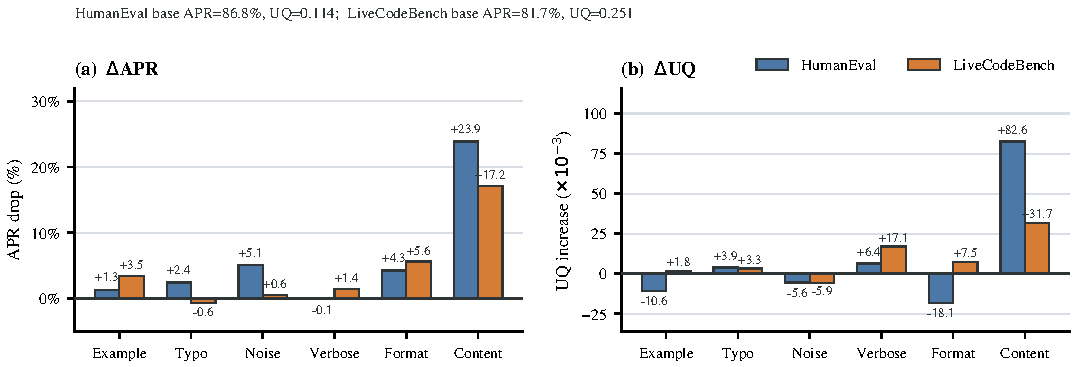
\includegraphics[width=1\textwidth]{preliminary_study_overview.pdf}
\caption{Impact of six requirement perturbation types on average pass-rate (APR) degradation and model-observed uncertainty (UQ) increase. $\Delta APR$ is computed as $APR_{\mathrm{orig}}-APR_{\mathrm{pert}}$ and $\Delta UQ$ is computed as $UQ_{\mathrm{pert}}-UQ_{\mathrm{orig}}$.}
\label{fig:preliminary-study-overview}
\end{figure*}

%explain the metric
\noindent \textbf{Metrics.} In this preliminary study, we set $K=5$ for repeated sampling. We evaluate code generation reliability using two complementary metrics: average pass rate, denoted as $APR$, and uncertainty quantification score, denoted as $UQ$. Our measurement of requirement uncertainty via code execution rests on a key assumption: since requirement uncertainty is not directly observable, we adopt generation inconsistency across repeated samples as a model-observed proxy. This assumption aligns with the existing work~\cite{mu2024clarifygpt, jia2025specfix}. 

Our intuition about uncertainty quantification is that an uncertain requirement may lead the model to generate programs that differ in implementation structure or behave inconsistently under the test suite. Accordingly, we consider two signals of generation inconsistency: structural inconsistency, which captures pairwise differences in generated code measured by CodeBLEU distance~\cite{ren2020codebleu}, and functional inconsistency, which captures variation in test execution outcomes across repeated samples.
We merge the metrics of these two views here to enhance comprehensiveness. 

Let $r_i$ denote the $i$-th requirement and $g_{ij}$ denote the $j$-th program generated for $r_i$ under repeated sampling, where $j\in{1,\ldots,K}$. We execute $g_{ij}$ against the corresponding test suite and define $t_{ij}\in[0,1]$ as the fraction of test cases passed. We compute the average pass rate of requirement $r_i$ as:
\begin{equation}
\label{eq:avgPassRate}
APR(r_i)=\frac{1}{K}\sum_{j=1}^{K}t_{ij}
\end{equation}
At the benchmark level, we report the mean $APR$ over all evaluated requirements, i.e., $\frac{1}{N}\sum_{i=1}^{N}APR(r_i)$.

While $APR(r_i)$ measures average functional correctness, it does not capture whether repeated generations implement the same requirement in structurally different ways. Therefore, we measure structural inconsistency using the average pairwise CodeBLEU distance among generated programs~\cite{ren2020codebleu}:
\begin{equation}
\label{eq:codebleuDistance}
D(r_i)=\frac{2}{K(K-1)}\sum_{1\leq a<b\leq K}
\left(1-\mathrm{CodeBLEU}(g_{ia},g_{ib})\right)
\end{equation}
A higher $D(r_i)$ indicates that repeated generations produce implementations with greater structural inconsistency for the same requirement.

However, structural inconsistency alone does not indicate whether the generated programs behave consistently under the test suite. Therefore, we further use the variation of test-case passing rates as an observable signal of functional inconsistency. Let $T_i={t_{i1},t_{i2},\ldots,t_{iK}}$ denote the set of passing rates observed under requirement $r_i$. We compute the variance of $T_i$ as:
\begin{equation}
\label{rq：passRateVariance}
\mathrm{Var}(T_i)=\frac{1}{K}\sum_{j=1}^{K}\left(t_{ij}-APR(r_i)\right)^2
\end{equation}
The functional inconsistency observed under $r_i$ is then defined as the normalized variance:
\begin{equation}
\label{eq:functionalInconsistency}
S(r_i)=\min\left(\frac{\mathrm{Var}(T_i)}{0.25}, 1\right)
\end{equation}
Since each $t_{ij}$ is bounded in $[0,1]$, we use the Bhatia--Davis inequality to bound the variance of the empirical passing-rate distribution~\cite{bhatia2000better}. Let $\mu_i=APR(r_i)$ denote the mean passing rate. The inequality gives
$$
\mathrm{Var}(T_i)\leq(1-\mu_i)(\mu_i-0)
=APR(r_i)(1-APR(r_i)).
$$
Since $APR(r_i)(1-APR(r_i))$ is maximized at $APR(r_i)=0.5$, we have $\mathrm{Var}(T_i)\leq0.25$. We therefore use $0.25$ as the normalization constant.


Finally, we compute the uncertainty score of requirement $r_i$ by equally combining structural and functional inconsistency:
\begin{equation}
\label{eq:uq}
UQ(r_i)=\frac{1}{2}\left(D(r_i)+S(r_i)\right)
\end{equation}
We report $APR$ separately as the correctness metric; therefore, $UQ$ focuses on generation inconsistency rather than directly incorporating average correctness. A larger $UQ$ value indicates higher model-observed requirement uncertainty.

Figure~\ref{fig:preliminary-study-overview} reports the impact of requirement perturbations on both HumanEval-ET and LiveCodeBench using the original requirements as the reference point. For each perturbation type, we report two relative metrics: average pass-rate degradation and uncertainty increase. Specifically, the former is computed as $\Delta APR=APR_{\mathrm{orig}}-APR_{\mathrm{pert}}$, where a positive value indicates that the perturbation reduces functional correctness. And the latter is computed as $\Delta UQ=UQ_{\mathrm{pert}}-UQ_{\mathrm{orig}}$, where a positive value indicates that the perturbation increases model-observed requirement uncertainty.


\begin{ellipsebox}
\centering
\normalfont\itshape
\textbf{Observation: Human-perceived perturbations do not uniformly translate into model-observed uncertainty.}
\end{ellipsebox}

Several surface-level perturbations have limited or inconsistent effects across benchmarks. For example, typographical perturbation leads to only a small increase in $UQ$ on both HumanEval-ET and LiveCodeBench, while noise injection even decreases $UQ$ in both settings. Verbose rewriting shows benchmark-dependent effects: it has almost no pass-rate impact on HumanEval-ET, but causes a clearer pass-rate drop and uncertainty increase on LiveCodeBench. These results suggest that perturbations that appear noisy or verbose from a human perspective are not necessarily the main source of model-observed uncertainty.

In contrast, content rewriting consistently causes the strongest degradation across both benchmarks. It leads to the largest $\Delta APR$ on HumanEval-ET and LiveCodeBench, and also produces the largest increase in $UQ$ on both datasets. This indicates that perturbations affecting the semantic expression of functional constraints, edge cases, or task intent are more likely to induce observable degradation and generation inconsistency than surface-level noise alone. Format transformation also shows non-negligible impact, especially in terms of pass-rate degradation, but its effect on $UQ$ is less consistent across benchmarks.

This observation carries an important implication for our study: requirement uncertainty should not be defined by whether a requirement appears ambiguous, noisy, or perturbed from a human perspective. Some perturbations that seem problematic to humans can be handled robustly by a strong code generation model, while others can induce clear correctness degradation or generation inconsistency. Therefore, in the following sections, we explore two directions: (1) how to annotate requirement uncertainty in a way that impact reliable code generation, and (2) how to proactively identify such uncertainty before code generation.

